\documentclass{article}

% Paquetes

\usepackage[utf8]{inputenc}
\usepackage{longtable}
\usepackage{authblk}
\usepackage{adjustbox}
\usepackage{natbib}

% Formalidades iniciales

\title{Proyecto de Integracion}

\author{\normalsize Daniel Bendeck De la Rosa}

\affil{\small Escuela de Ingenieria,Universidad de los Andes\\Bogota, Colombia}

\date{29 de Junio de 2018}

\usepackage{Sweave}
\begin{document}
\Sconcordance{concordance:ProyectoFinal.tex:ProyectoFinal.Rnw:%
1 20 1 1 0 9 1 1 13 16 1 1 4 15 0 1 2 12 1 1 12 1 2 11 1 1 5 12 0 1 2 2 %
1 1 7 13 0 1 2 2 1 2 2 8 1 2 5 31 0 1 2 8 1 1 8 1 39 3 1 1 9 1 2 9 1}


\maketitle

% Cargar archivo ----

%

% NO OLVIDAR set working directory

\begin{abstract}
Este es mi primer trabajo en exploracion y construccion de documentos a partir de la herramienta LATEX. 
\end{abstract}

% Exploracion Univariada --------------------------------------------------

\section{Exploracion Univariada}\label{univariada}

En esta seccion exploro cada indice.\\

Para conocer el comportamiento de las variables se ha preparado la Tabla \ref{stats}, donde se describe la distribucion de las modalidades de cada variable. Los numeros representan la situacion de algun pais en ese indicador, donde el mayor valor numerico es la mejor situacion.

%% estadisticos

Nos interesa IDH, y poblacion cabecera y poblacion resto no se puede secar tabla de frecuencia, solo estadisticos:

% Table created by stargazer v.5.2.2 by Marek Hlavac, Harvard University. E-mail: hlavac at fas.harvard.edu
% Date and time: Fri, Jun 29, 2018 - 20:16:08
\begin{table}[!htbp] \centering 
  \caption{Medidas estadisticas} 
  \label{stats} 
\begin{tabular}{@{\extracolsep{5pt}}lccccc} 
\\[-1.8ex]\hline 
\hline \\[-1.8ex] 
Statistic & \multicolumn{1}{c}{N} & \multicolumn{1}{c}{Min} & \multicolumn{1}{c}{Median} & \multicolumn{1}{c}{Mean} & \multicolumn{1}{c}{Max} \\ 
\hline \\[-1.8ex] 
IDH & 32 & 0.691 & 0.804 & 0.802 & 0.879 \\ 
Poblacion.Cabecera & 32 & 13,090 & 717,197 & 1,196,730.000 & 10,070,801 \\ 
Poblacion.Resto & 32 & 21,926 & 268,111.5 & 360,590.300 & 1,428,858 \\ 
Poblacion.Total & 32 & 43,446 & 1,028,429 & 1,557,320.000 & 10,985,285 \\ 
\hline \\[-1.8ex] 
\end{tabular} 
\end{table} \label{stats}

Como apreciamos en la Tabla \ref{stats}, los paises en la mejor situacion son los menos, salvo en el caso del \emph{indice de libertad mundial}\footnote{Notese que esto se puede deber a la {\bf menor} cantidad de categorias.}

\clearpage

Para resaltar lo anterior, tenemos la Figura \ref{pintarHistogramas} en la pagina \pageref{pintarHistogramas}. 

%% graficos
\begin{figure}[h]
\centering

El plot de cada uno seria el histograma:
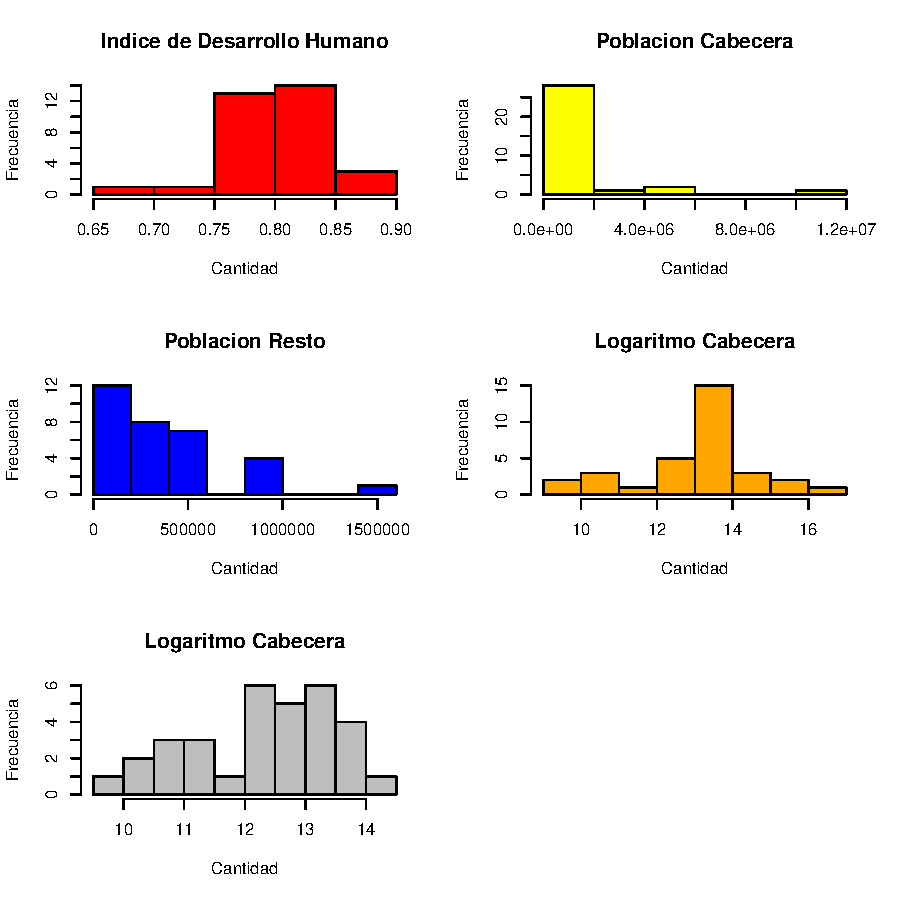
\includegraphics{ProyectoFinal-pintarHistogramas}
\caption{Distribucion de Indicadores}
\label{pintarHistogramas}
\end{figure}

\clearpage

% Exploracion Bivariada ---------------------------------------------------

\section{Exploracion Bivariada}\label{Bivariada}

En este trabajo estamos interesados en el impacto de la poblacion en el el IDH, veamos IDH con cada uno:

% Table created by stargazer v.5.2.2 by Marek Hlavac, Harvard University. E-mail: hlavac at fas.harvard.edu
% Date and time: Fri, Jun 29, 2018 - 20:16:08
\begin{table}[!htbp] \centering 
  \caption{Correlacion Democracia con las variables restantes} 
  \label{corrDem} 
\begin{tabular}{@{\extracolsep{5pt}} cc} 
\\[-1.8ex]\hline 
\hline \\[-1.8ex] 
cabeLog & restoLog \\ 
\hline \\[-1.8ex] 
$0.487$ & $0.177$ \\ 
\hline \\[-1.8ex] 
\end{tabular} 
\end{table} 
A continuacion la correlacion entre las variables independientes:

% Table created by stargazer v.5.2.2 by Marek Hlavac, Harvard University. E-mail: hlavac at fas.harvard.edu
% Date and time: Fri, Jun 29, 2018 - 20:16:08
\begin{table}[!htbp] \centering 
  \caption{Correlacion Democracia con las variables independientes} 
  \label{corrTableX} 
\begin{tabular}{@{\extracolsep{5pt}} ccc} 
\\[-1.8ex]\hline 
\hline \\[-1.8ex] 
 & cabeLog & restoLog \\ 
\hline \\[-1.8ex] 
cabeLog & 1 &  \\ 
restoLog & 0.84 & 1 \\ 
\hline \\[-1.8ex] 
\end{tabular} 
\end{table}  
Visualmente podemos ver el comportamiento de las correlaciones a continuacion:

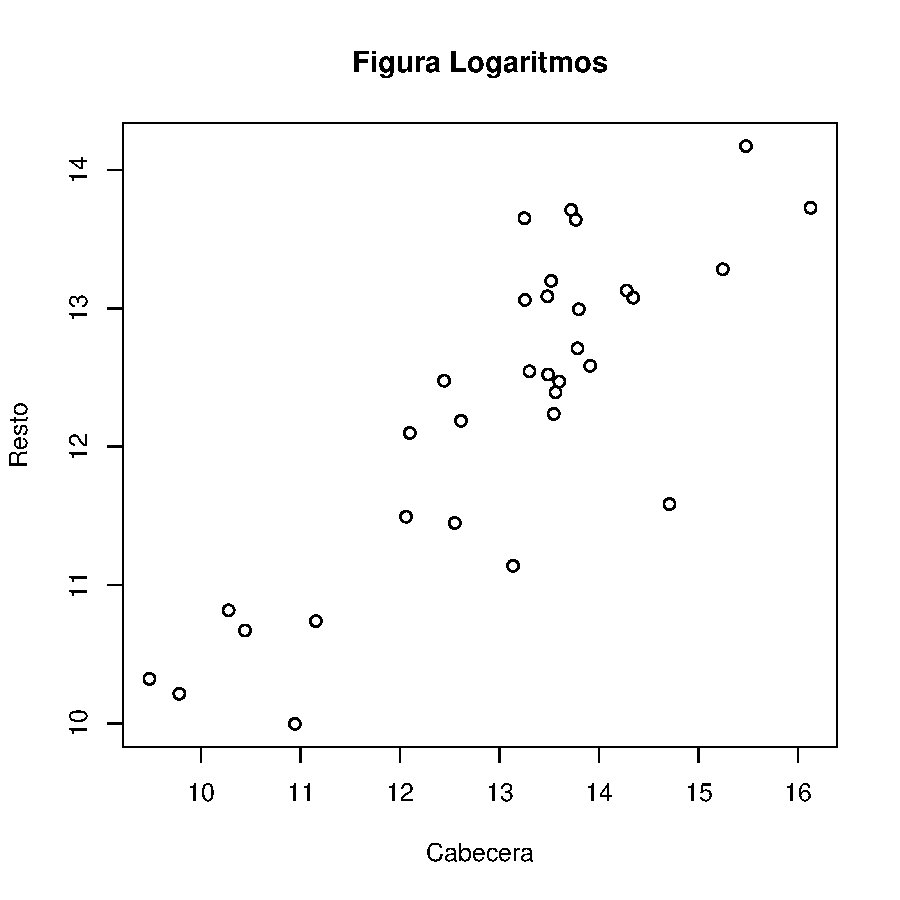
\includegraphics{ProyectoFinal-verCorr}

\clearpage

% Modelos de Regresi<U+00F3>n ----------------------------------------------------

\section{Modelos de Regresion}\label{Regresion}

Veamos los modelos propuestos. \\
Primero sin poblacion resto, luego con esta:

% Table created by stargazer v.5.2.2 by Marek Hlavac, Harvard University. E-mail: hlavac at fas.harvard.edu
% Date and time: Fri, Jun 29, 2018 - 20:16:08
\begin{table}[!htbp] \centering 
  \caption{Modelos de Regresion} 
  \label{regresion} 
\begin{tabular}{@{\extracolsep{5pt}}lcc} 
\\[-1.8ex]\hline 
\hline \\[-1.8ex] 
 & \multicolumn{2}{c}{\textit{Dependent variable:}} \\ 
\cline{2-3} 
\\[-1.8ex] & \multicolumn{2}{c}{IDH} \\ 
\\[-1.8ex] & (1) & (2)\\ 
\hline \\[-1.8ex] 
 cabeLog & 0.013$^{***}$ & 0.031$^{***}$ \\ 
  & (0.004) & (0.007) \\ 
  & & \\ 
 restoLog &  & $-$0.030$^{***}$ \\ 
  &  & (0.010) \\ 
  & & \\ 
 Constant & 0.634$^{***}$ & 0.766$^{***}$ \\ 
  & (0.055) & (0.065) \\ 
  & & \\ 
\hline \\[-1.8ex] 
Observations & 32 & 32 \\ 
R$^{2}$ & 0.238 & 0.425 \\ 
Adjusted R$^{2}$ & 0.212 & 0.385 \\ 
Residual Std. Error & 0.037 (df = 30) & 0.033 (df = 29) \\ 
F Statistic & 9.347$^{***}$ (df = 1; 30) & 10.706$^{***}$ (df = 2; 29) \\ 
\hline 
\hline \\[-1.8ex] 
\textit{Note:}  & \multicolumn{2}{r}{$^{*}$p$<$0.1; $^{**}$p$<$0.05; $^{***}$p$<$0.01} \\ 
\end{tabular} 
\end{table} 
\clearpage

%Exploracion Espacial ----------------------------------------------------

\section{Exploracion Espacial}\label{Exporacion}

Calculemos conglomerados de regiones, usando toda la informacion de las tres variables.Usaremos la tecnica de k-means {\bf Mc Queen} propuesta por MacQueen en \cite{gower_general_1971}. Los tres conglomerados se muestran en la Figura \ref{clustmap}.



\begin{figure}[h]
\centering

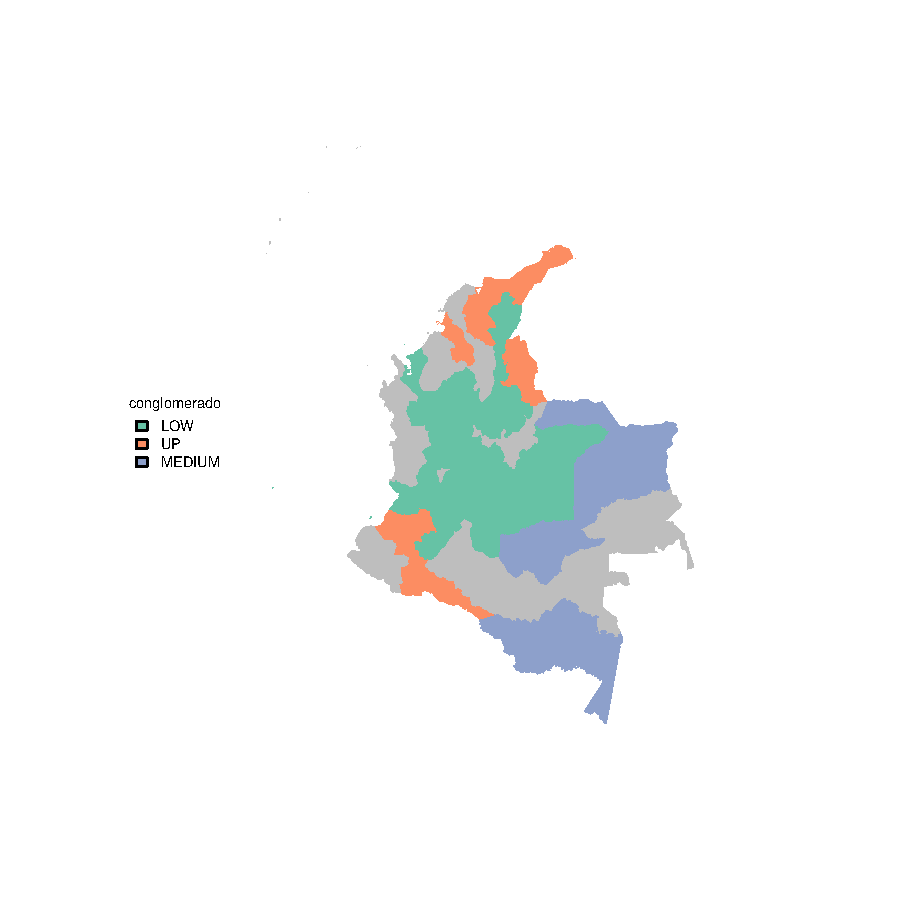
\includegraphics{ProyectoFinal-plotMap1}
%\end{adjustbox}
\caption{Departamentos Conglomerados y su IDH}
\label{clustmap}
\end{figure}

\bibliographystyle{apalike}
\renewcommand{\refname}{Bibliografia}
\bibliography{BibProyecto}

\end{document}
